\documentclass[12pt]{article}
\usepackage{graphicx}
\usepackage{hyperref}
\usepackage[top=2.75in, left=1in, right=1in, bottom=0.25in]{geometry}
\usepackage[utf8]{inputenc}
\usepackage[english]{babel}
\usepackage{fancyhdr}
\usepackage[utf8]{inputenc}
\usepackage{listings}
\usepackage{color}
\usepackage[final]{pdfpages}
\usepackage{multirow}
\usepackage{array}
\usepackage{caption}
\usepackage{subcaption}

\definecolor{codegreen}{rgb}{0,0.6,0}
\definecolor{codegray}{rgb}{0.5,0.5,0.5}
\definecolor{codepurple}{rgb}{0.58,0,0.82}
\definecolor{backcolour}{rgb}{0.95,0.95,0.92} 
\lstdefinestyle{mystyle}{
    backgroundcolor=\color{backcolour},   
    commentstyle=\color{codegreen},
    keywordstyle=\color{magenta},
    numberstyle=\tiny\color{codegray},
    stringstyle=\color{codepurple},
    basicstyle=\footnotesize,
    breakatwhitespace=false,         
    breaklines=true,                 
    captionpos=b,                    
    keepspaces=true,                 
    numbers=left,                    
    numbersep=5pt,                  
    showspaces=false,                
    showstringspaces=false,
    showtabs=false,                  
    tabsize=2
} 
\lstset{style=mystyle}

\setlength{\parindent}{4em}
\setlength{\parskip}{1em}
\pagestyle{fancy}
\fancyhf{}
\rhead{Assignment 8}
\lhead{Huan Huang}
\renewcommand{\headrulewidth}{0.4pt}
\renewcommand{\footrulewidth}{0.4pt}
\rfoot{Page \thepage}


\begin{document}
\begin{titlepage}
	\begin{center}
	\Huge{Web Science cs532-s16}\\
	[0.25in]
	\textsc{\Large Assignment 8 Report}\\
	\textsc{\normalsize Dr. Michael L. Nelson}\\
	[4.25in]
	\textsc{\normalsize By: Huan Huang}\\
	\large 04/07/2016\\
	
	
	\end{center}
\end{titlepage}
\newpage

\newgeometry{margin=1in}


\section*{Problem 1}

\noindent
Create a blog-term matrix.  Start by grabbing 100 blogs; include:

\begin{verbatim}
http://f-measure.blogspot.com/
http://ws-dl.blogspot.com/
\end{verbatim}

and grab 98 more as per the method shown in class.  Note that this
method randomly chooses blogs and each student will separately do
this process, so it is unlikely that these 98 blogs will be shared
among students.  In other words, no sharing of blog data.  Upload
to github your code for grabbing the blogs and provide a list of
blog URIs, both in the report and in github..

Use the blog title as the identifier for each blog (and row of the
matrix).  Use the terms from every item/title (RSS) or entry\/title
(Atom) for the columns of the matrix.  The values are the frequency
of occurrence.  Essentially you are replicating the format of the
``blogdata.txt" file included with the PCI book code.  Limit the
number of terms to the most ``popular" (i.e., frequent) 500 terms,
this is *after* the criteria on p. 32 (slide 7) has been satisfied.


\subsection*{Answer}
To solve this problem, I first wrote a shell script to click on the next-blog button for 397 times, then, the 397 final URIs I got are saved together with the 2 required links in a file.

\begin{figure}[h]
\centering
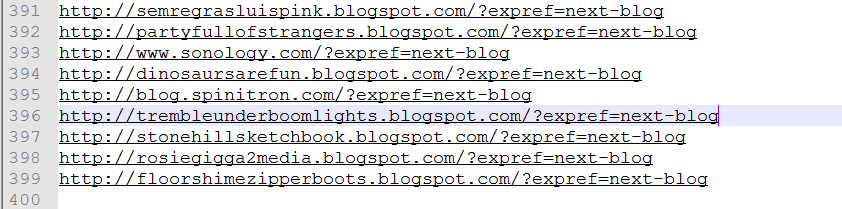
\includegraphics[width=6.5in]{blogList.png}
\caption{Sample of part of blogList.txt}
\end{figure}

\lstinputlisting[language=bash]{getblogs.sh}

The reason I apply the next-blog link 397 times is because it often give me the same blog pages. Therefore, I use the command ``sort -u filename" to remove the duplicate URIs and saved the result in the file unique.txt. 

\begin{figure}[h]
\centering
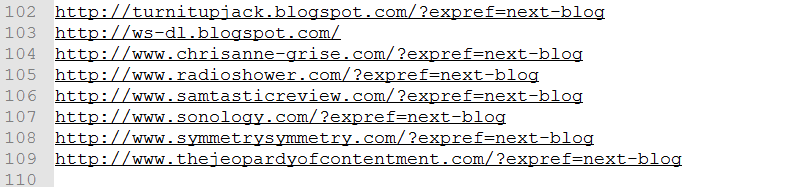
\includegraphics[width=6.5in]{unique.png}
\caption{Sample of part of unique.txt}
\end{figure}

Once I have the unique links, I use another shell script to get the atom feed URIs of each of the unique links in the file unique.txt. Then, remove the extra links to make sure there are exactly 100 of them.

\begin{figure}[h]
\centering
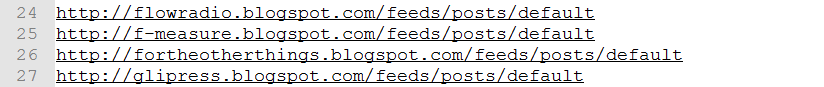
\includegraphics[width=6.5in]{atomf.png}
\caption{Sample of part of atom.txt}
\end{figure}
\begin{figure}[h]
\centering
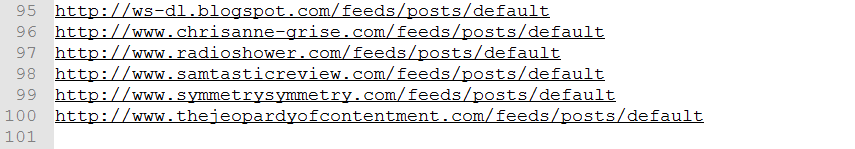
\includegraphics[width=6.5in]{atomm.png}
\caption{Another sample of part of atom.txt}
\end{figure}

\lstinputlisting[language=bash]{getAtom.sh}

Now, I use the generatefeedvector.py file I collected from the PCI(Programming Collective Intelligence) book to generate the word count file called blogdata.txt. I modified the generatefeedvector.py file slightly to count only 500 popular terms. 

\begin{figure}[h]
\centering
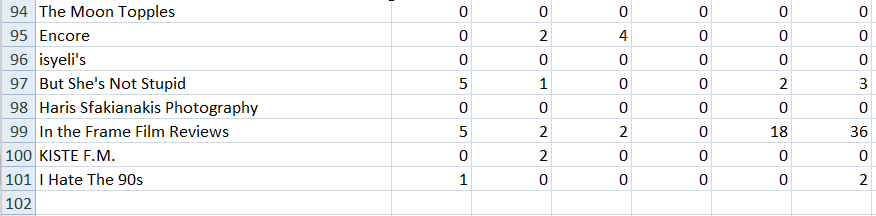
\includegraphics[width=6.5in]{blogdata.png}
\caption{Sample of part of blogdata.txt}
\end{figure}

\lstinputlisting[language=python]{generatefeedvector.py}

\section*{Problem 2}

Create an ASCII and JPEG dendrogram that clusters (i.e., HAC)
the most similar blogs (see slides 12 \& 13).  Include the JPEG in
your report and upload the ascii file to github (it will be too
unwieldy for inclusion in the report).

\subsection*{Answer}
For this problem, I imported another file called cluster.py from PCI codes. Then, call the functions readfile() to process the data in blogdata.txt to get necessary information to feed to another function called hcluster(). The function hcluster() uses Person's method to decide which blogs are grouped together, then the clusters are plotted  by another function called printclust() based on the result from hcluster(). Lastly, the image is drawn by the drawdendrogram() function. 

\lstinputlisting[language=python]{clusters.py}
\lstinputlisting[language=python]{bloghclusters.py}

\begin{figure}
\centering
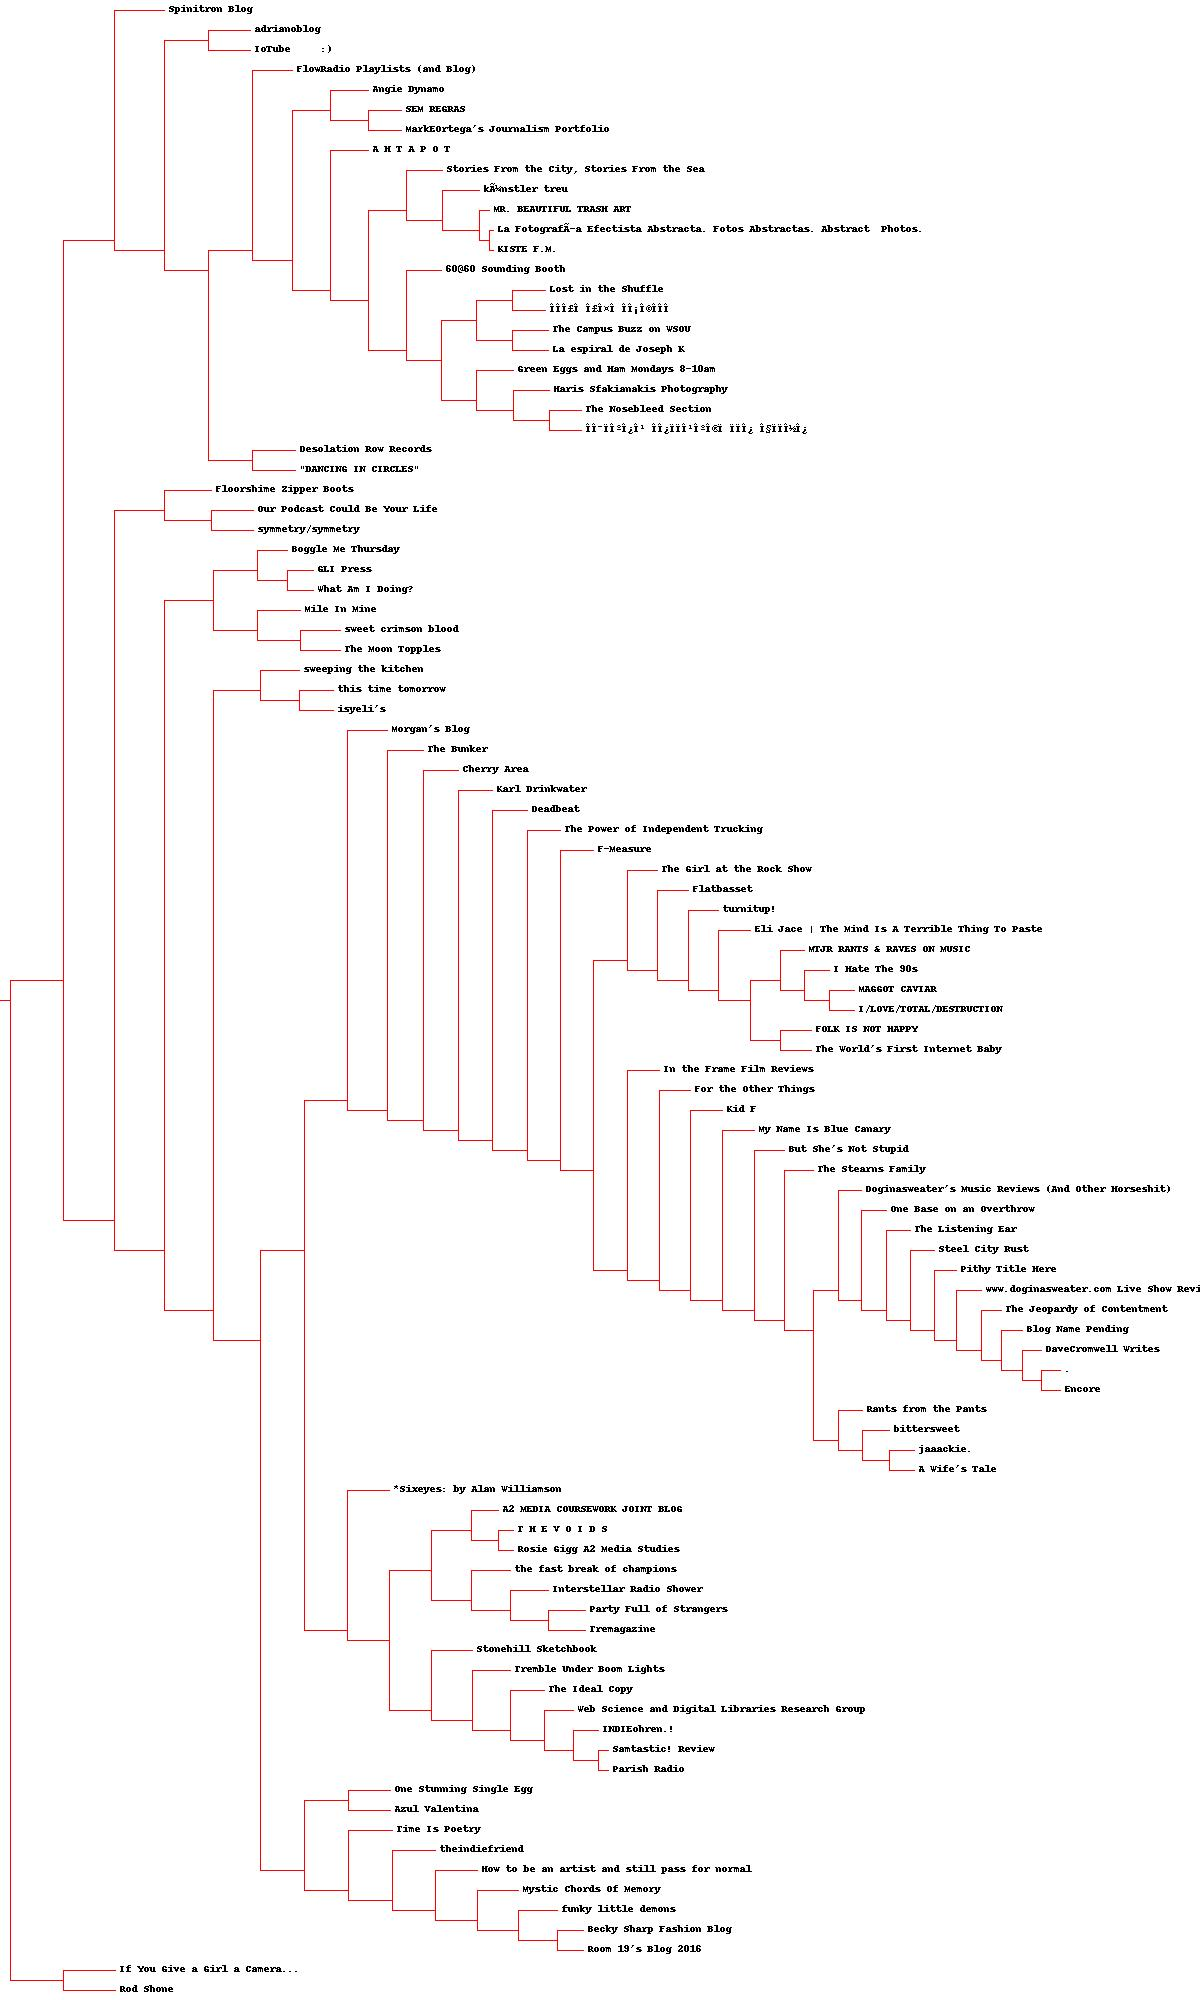
\includegraphics[width=5in]{blogclust.jpg}
\caption{The dendrogram of clusters of 100 blog pages}
\end{figure}
\pagebreak

\section*{Problem 3}

Cluster the blogs using K-Means, using k=5,10,20. (see slide
18).  Print the values in each centroid, for each value of k. How
many interations were required for each value of k?

\subsection*{Answer}

To solve this problem, I just wrote a short python code to call for the necessary functions in cluster.py and print out the information needed. Below is just a sample of part of the result, to see the full list please check the kcentroid.txt file in folder Problem3 on my github account. 

\begin{figure}[h]
\centering
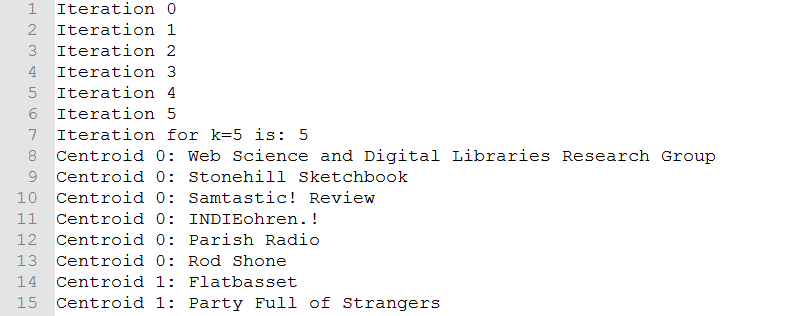
\includegraphics[width=6.5in]{kcentroid.png}
\caption{Sample of part of kcentroid.txt}
\end{figure}
\pagebreak

\lstinputlisting[language=python]{blogkcluster.py}
\pagebreak

\section*{Problem 4}

Use MDS to create a JPEG of the blogs similar to slide 29.  
How many iterations were required?

\subsection*{Answer}

Again, I just called for the necessary functions in cluster.py to solve this problem. The functions need for this problem are:\\
readfile() - to process the data in blogdata.txt\\
scaledown() - to calculate the distance of the points and iterate\\
draw2d() - to draw the image based on the result from scaledown()

\begin{figure}[h]
\centering
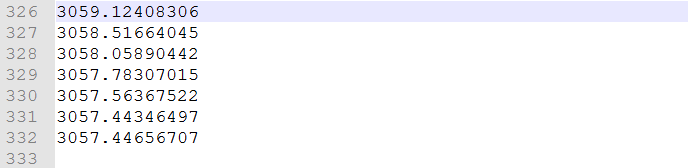
\includegraphics[width=6.5in]{scaledowniterations.png}
\caption{Sample of part of scaledowniterations.txt}
\end{figure}

As you can see, the program stopped at iteration 332, because after iteration 331, the error value starts to increase.

\lstinputlisting[language=python]{MDS.py}

\begin{figure}[h]
\centering
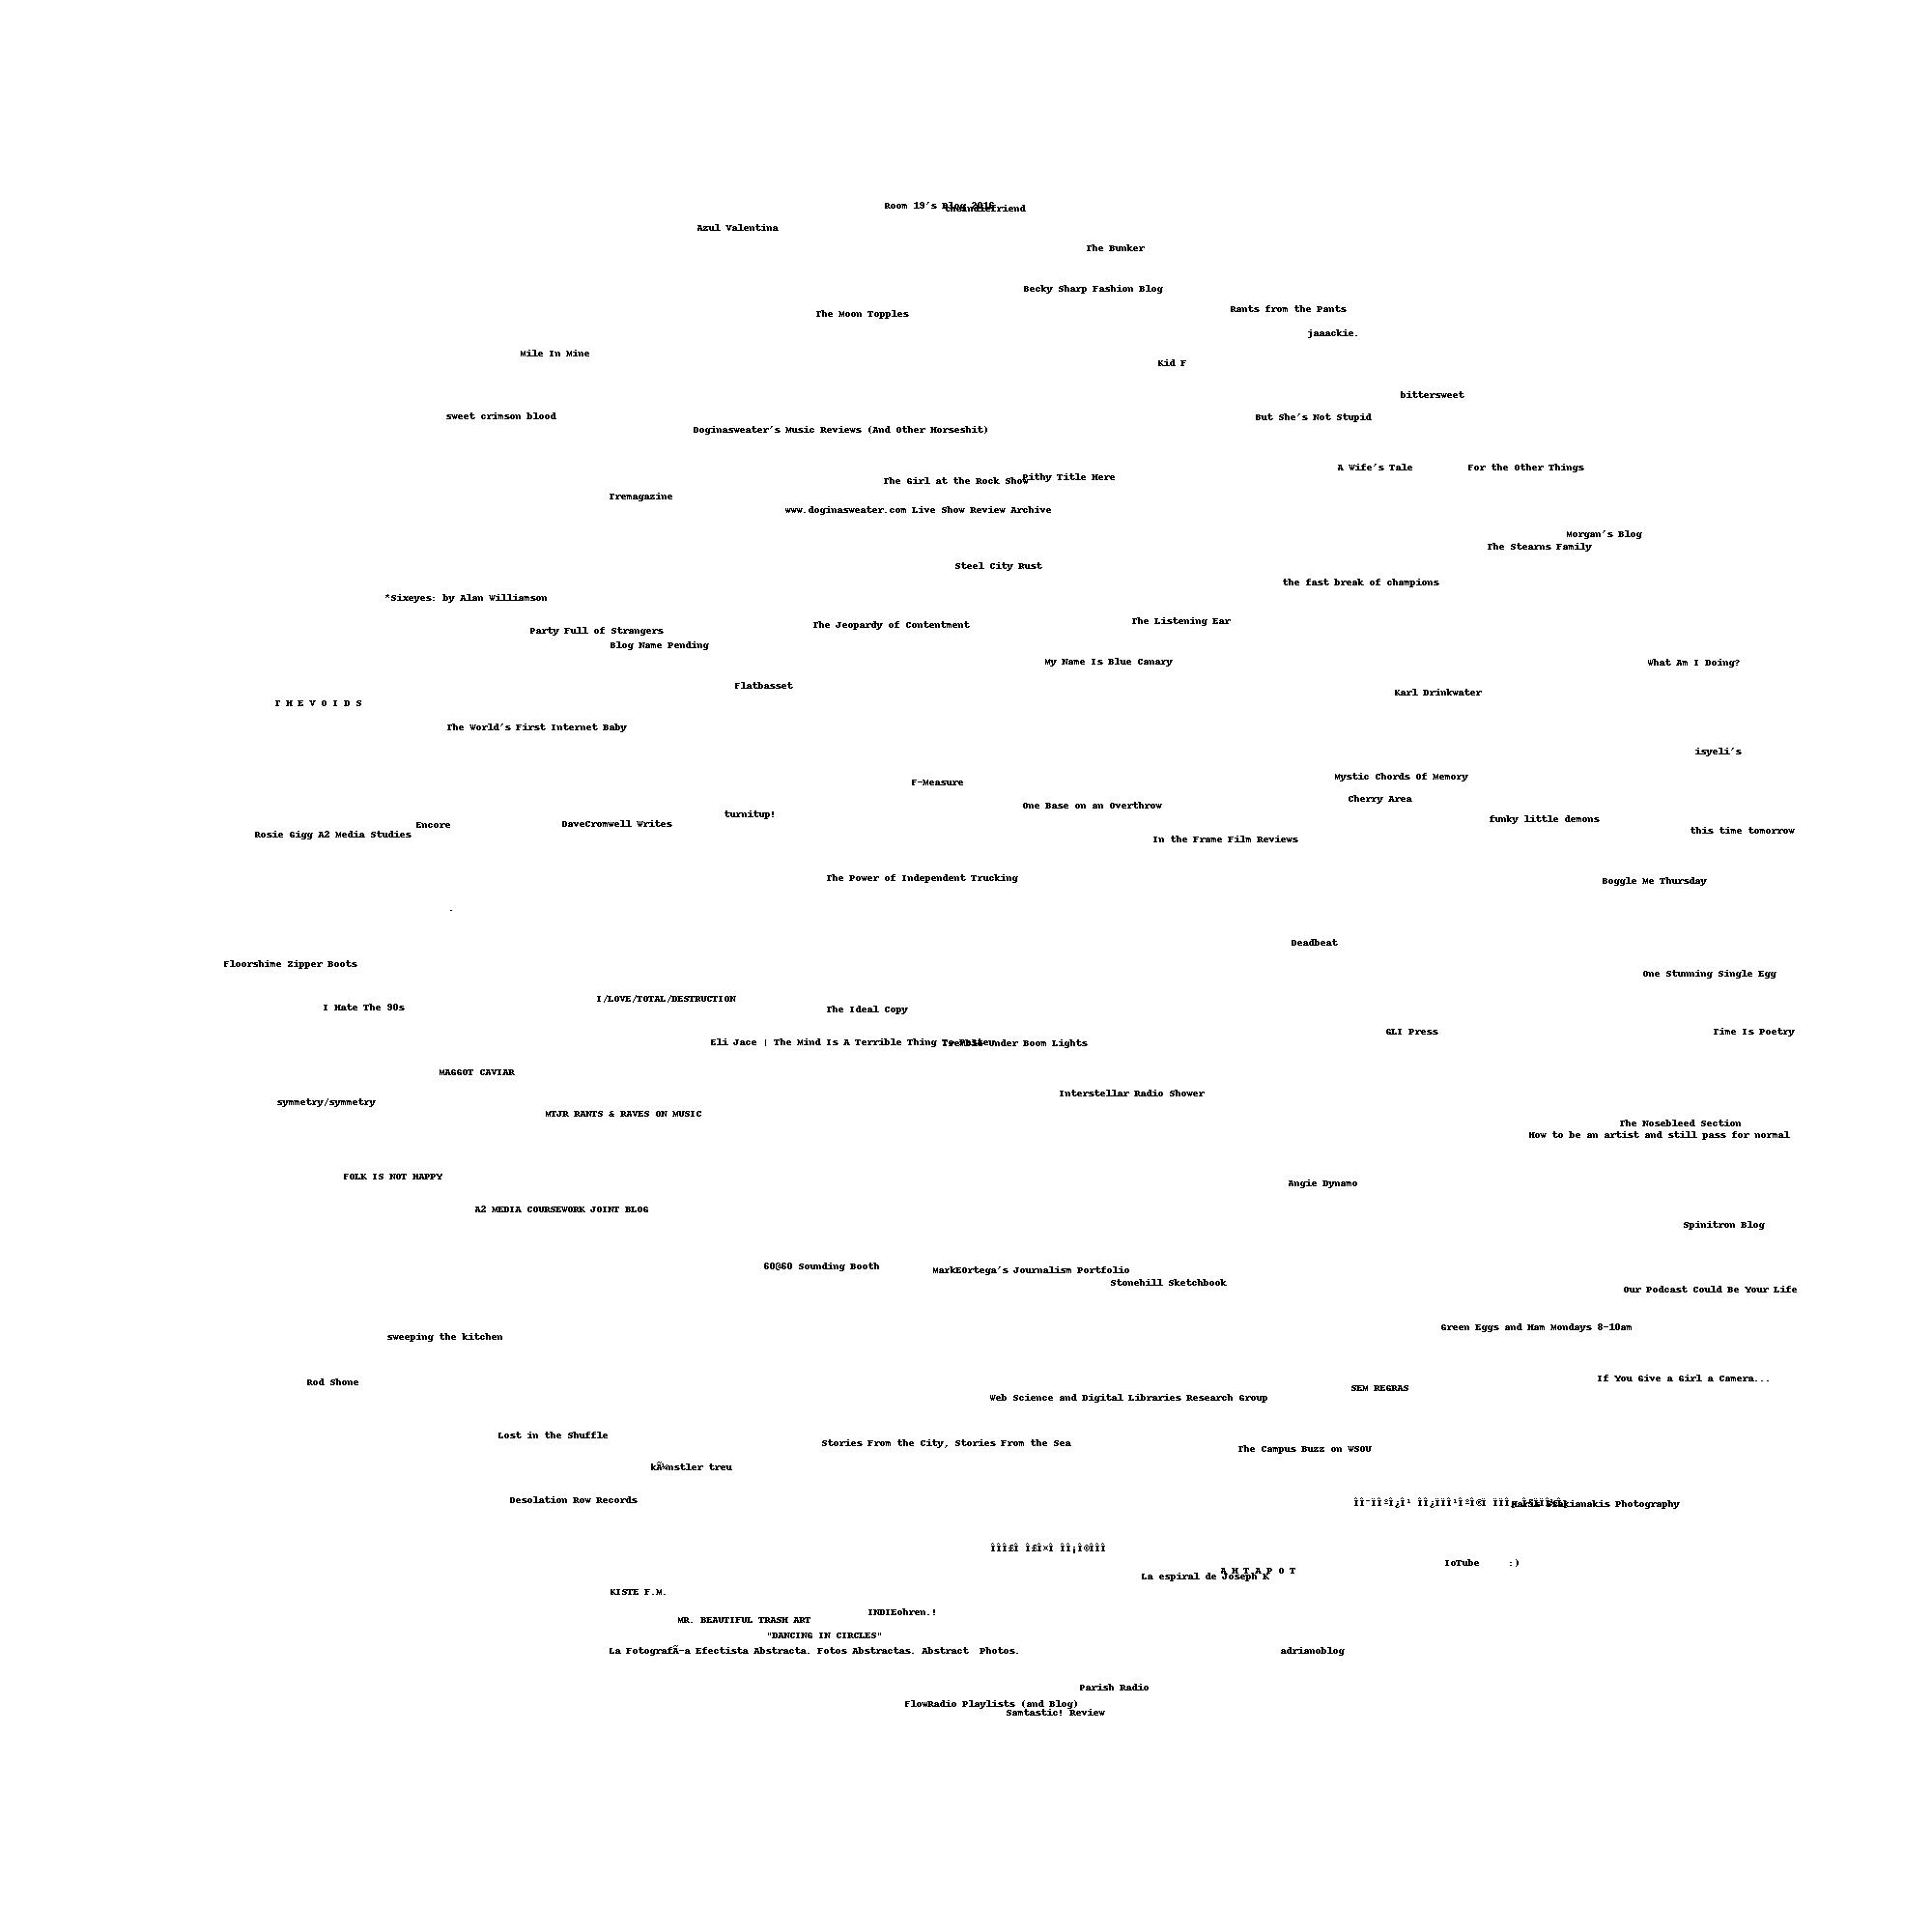
\includegraphics[width=6.5in]{MDS.jpg}
\caption{Image of the 100 blog pages based on the Multidimensional Scaling}
\end{figure}
\pagebreak



\end{document}